\section{Improvement journey}

The final model came out of a sequence of experiments. Each step changed one idea, motivated by what the previous
step got wrong. All six steps were re-run on the same five development folds for this report
(Table~\ref{tab:ladder}, Figure~\ref{fig:ladder}).

\begin{enumerate}
  \item \textbf{Equipment rate per mile $\times$ distance} (\usd{\DevStepA}). The simplest sensible price. It knows
        nothing about place, weight or time.
  \item \textbf{CatBoost on raw dollars} (\usd{\DevStepB}). The original submission. It learns place and weight but
        fits dollars with a squared loss, so the corrupted labels pull it around, and its month features never saw a
        December.
  \item \textbf{LightGBM on log rate with the label screen, market and calendar} (\usd{\DevStepC}). Working on the
        log scale and dropping corrupted labels fix step 2's two worst problems. But trees cannot extend a trend or a
        market level beyond what they saw, so errors stay large when the level moves.
  \item \textbf{Structural ridge} (\usd{\DevStepD}). Time and market enter as straight lines on the log scale, so
        they extrapolate. This step removes most of the remaining error.
  \item \textbf{Ridge plus residual trees} (\usd{\DevStepE}). A small LightGBM learns the local patterns the ridge
        misses, such as a lane's geography interacting with distance and weight.
  \item \textbf{Tuned and recency-weighted} (\usd{\DevStepF}). Tuned spline knots and a larger, slower tree stage
        (Section~\ref{sec:tuning}). Recent loads weigh more, with a time constant of \RecencyTau{} days.
\end{enumerate}

\begin{table}[H]
  \caption{The improvement ladder on the five development folds. ``Change'' is relative to the previous step.}
  \label{tab:ladder}
  \inputtable{ladder}
\end{table}

\begin{figure}[H]
  \centering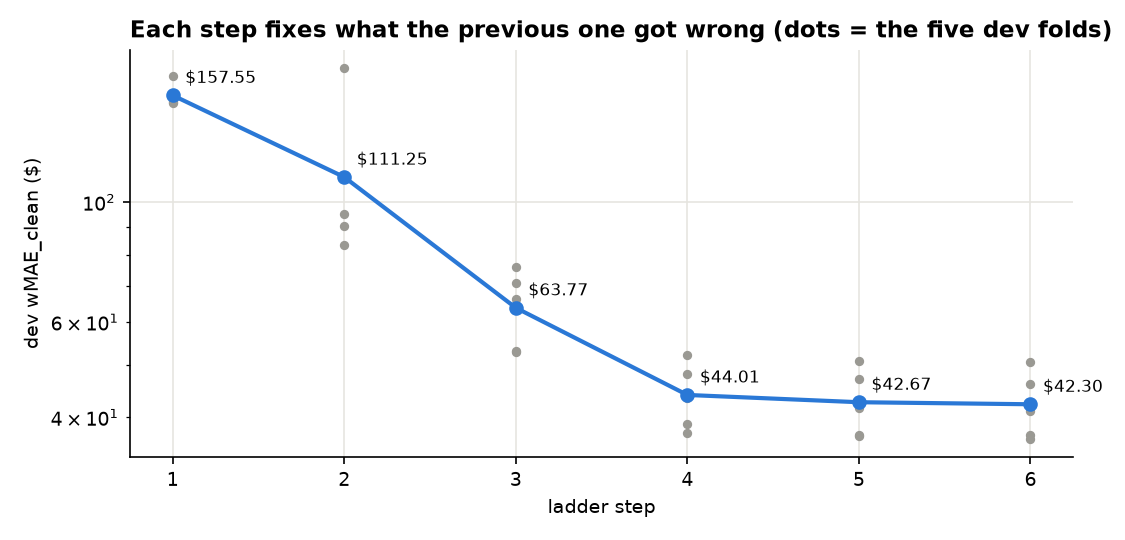
\includegraphics[width=0.85\linewidth]{ladder.png}
  \caption{Development error by ladder step (log scale). Grey dots are the five folds.}\label{fig:ladder}
\end{figure}

Simple time-series baselines sit between steps 2 and 3. The best of them, a cross-section model with the last
daily price level carried forward, scores \usd{\DevNaiveIndex} (Table~\ref{tab:baselines}).

\begin{table}[H]
  \caption{Baselines on the development folds.}\label{tab:baselines}
  \inputtable{baselines}
\end{table}

\begin{table}[H]
  \caption{Paired 7-day block-bootstrap comparisons on the development folds (final minus other model;
  negative means the final model is better).}\label{tab:devci}
  \inputtable{dev_comparisons}
\end{table}
